\documentclass{article} 

\usepackage{fancyhdr}
\usepackage[english]{babel}

\usepackage{fullpage}
\usepackage[margin = .75 in]{geometry}
\usepackage[leqno]{amsmath}
\usepackage{amsfonts}
\usepackage{amssymb}
\usepackage{amsthm}
\usepackage{amssymb}
\usepackage[all]{xy}
\usepackage{graphicx}

\usepackage{graphicx,color,url,hyperref}
\usepackage{epsfig}
\fancyhf{}
\setlength{\parindent}{0pt}
\setlength{\parskip}{5pt plus 1pt}
\setlength{\headheight}{13.6pt}

\newcommand{\NN}{\mathbf N}
\newcommand{\RR}{\mathbf R}
\newcommand{\CC}{\mathbf C}
\newcommand{\ZZ}{\mathbf Z}
\newcommand{\ZZn}[1]{\ZZ/{#1}\ZZ}
\newcommand{\QQ}{\mathbf Q}
\newcommand{\nn}{\mathbb N}
\newcommand{\rr}{\mathbb R}
\newcommand{\cc}{\mathbb C}
\newcommand{\zz}{\mathbb Z}
\newcommand{\zzn}[1]{\zz/{#1}\zz}
\newcommand{\qq}{\mathbb Q}
\newcommand{\calM}{\mathcal M}
\newcommand{\latex}{\LaTeX}
\newcommand{\tex}{\TeX}
\newcommand{\dd}{{\rm d}}
\newcommand{\sm}{\setminus} 

\title{Worksheet 1}
\author{Sunny Lee}
\date{February 23, 2021}

\pagestyle{fancy}
\fancyhf{}
\rhead{February 23, 2021}
\lhead{Sunny Lee}
\chead{Homework 1}
\rfoot{Page \thepage}

\begin{document}

\begin{enumerate}
    \item Let $(a_n)$ be a seqence which converges to a limit L. Then, by definition, 
    there exists $N \in \NN$ such that if $n\geq N$, $|a_n - L| < \epsilon$. Since 
    $b_n = \frac{1}{n}(a_1 + a_2 + \cdots + a_n)$, if $n\geq N$, $b_n = \frac{1}{n}
    (a_1 + a_2 + \cdots + a_{N-1}) + \frac{1}{n}(a_{N} + \cdots + a_{n-1} + a_{n})$.
    Then, $b_n \leq |b_n| = |\frac{1}{n}
    (a_1 + a_2 + \cdots + a_{N-1}) + \frac{1}{n}(a_{N} + \cdots + a_{n-1} + a_{n})|
    \leq |\frac{1}{n}
    (a_1 + a_2 + \cdots + a_{N-1})| + |\frac{1}{n}(a_{N} + \cdots + a_{n-1} + a_{n}))|$. 
    Then, since $|a_n - L| < \epsilon$, the max value $a_n$ can take is $L+\epsilon$ 
    for all $n \geq N$. Thus, $|\frac{1}{n}(a_{N} + \cdots + a_{n-1} + a_{n}))| < 
    |\frac{(n-N)(L+\epsilon)}{n}| < L+\epsilon$. Thus, $b_n < |\frac{1}{n}
    (a_1 + a_2 + \cdots + a_{N-1})| + L + \epsilon$ which is a finite number. Therefore, 
    at some point $b_n$ must converge. 

    \item Without loss of generality, assume $a > b$. Then since $a > b$, $(a^n + b^n)^{1/n}
    < (2a^n)^{1/n}$ and $(a^n)^{1/n} < (a^n + b^n)^{1/n}$. Then, $a < (a^n + b^n)^{1/n}
    < (2a^n)^{1/n} = 2^{1/n}a$ and as $n\rightarrow \infty$, $a < (a^n + b^n)^{1/n}
    < a$ and thus, by the squeeze theorem $(a^n + b^n)^{1/n} \rightarrow a$. 

    \item Let $\frac{1}{2} < \epsilon$. Claim: $|\sqrt{n+1} - \sqrt{n} - 0| < \epsilon$.
    Since, $\sqrt{n+1} - \sqrt{n} = \frac{1}{\sqrt{n+1}+\sqrt{n}}$.  
    Since $\sqrt{n+1}+\sqrt{n} > 2\sqrt{n}$, $\frac{1}{\sqrt{n+1}+\sqrt{n}} 
    < \frac{1}{2\sqrt{n}}$. Since $n\geq 1$, and $\frac{1}{2\sqrt{n}} > \frac{1}{2\sqrt{n+1}}$, 
    $\frac{1}{2\sqrt{n}} < \frac{1}{2} < \epsilon$. Thus, $|\sqrt{n+1} - \sqrt{n} - 0| < \epsilon$, 
    thus $\lim_{n\rightarrow \infty} \sqrt{n+1} - \sqrt{n} = 0$. 

    \item Assume $\lim_{n\rightarrow \infty} x_n = x $ and $ \lim_{n\rightarrow \infty} y_n = y$ 
    Then, $|(x_n + y_n) - (x + y)| = |x_n - x + y_n - y| \leq |x_n - x| + |y_n - y|$. Since
    $(x_n)\rightarrow x$ and $(y_n)\rightarrow y$, we can find $N_1, N_2$ such that
    $|x_n - x| <\frac{\epsilon}{2}, \forall n\geq N_1$. and 
    $|y_n - y| <\frac{\epsilon}{2}, \forall n\geq N_2$. Thus, if we take $N = max\{N_1, N_2\}$, 
    we get that $|(x_n + y_n) - (x + y)| \leq |x_n - x| + |y_n - y| = \epsilon$. 

    \item Let $\{a_n\}$ be a sequence of real numbers such that $|a_n| \leq 2$ and 
    $|a_{n+2} - a_{n+1}| \leq \frac{1}{8}|a_{n+1}^2 - a_n^2| \forall n\geq 1$. Then, 
    $\frac{1}{8}|a_{n+1}^2 - a_n^2| = \frac{1}{8}|(a_{n+1} - a_n)(a_{n+1} + a_n)|
    \leq \frac{1}{8^2}|a_n^2 - a_{n-1}^2||a_{n+1} + a_n| \leq \cdots \leq 
    \frac{1}{8^{n-2}}|a_2^2 - a_1^2||a_{n+1}+a_n|\cdots |a_3 + a_2|$. 
    Since $|a_n|\leq 2$, $\frac{1}{8^{n-2}}|a_2^2 - a_1^2||a_{n+1}+a_n|\cdots |a_3 + a_2|
    \leq \frac{1}{8^{n-2}}|a_2^2 - a_1^2||2+2|\cdots |2 + 2| = 
    \frac{1}{8^{n-2}}|a_2^2 - a_1^2|4^{n-2} = \frac{1}{2^{n-2}}|a_2^2 - a_1^2|$. Since 
    $\frac{1}{2^{n-2}}\rightarrow 0$ as $n\rightarrow \infty$, $\{a_n\}$ is Cauchy. Thus
    $\{a_n\}$ converges. 

    \item Using matlab:\\ 
    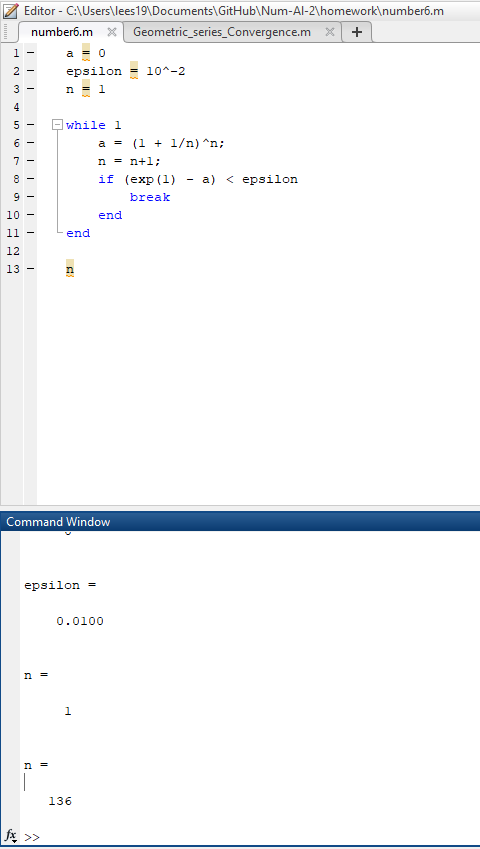
\includegraphics[scale = .8]{a.png}\\
    We find that this sequence does indeed converge to $e$: \\
    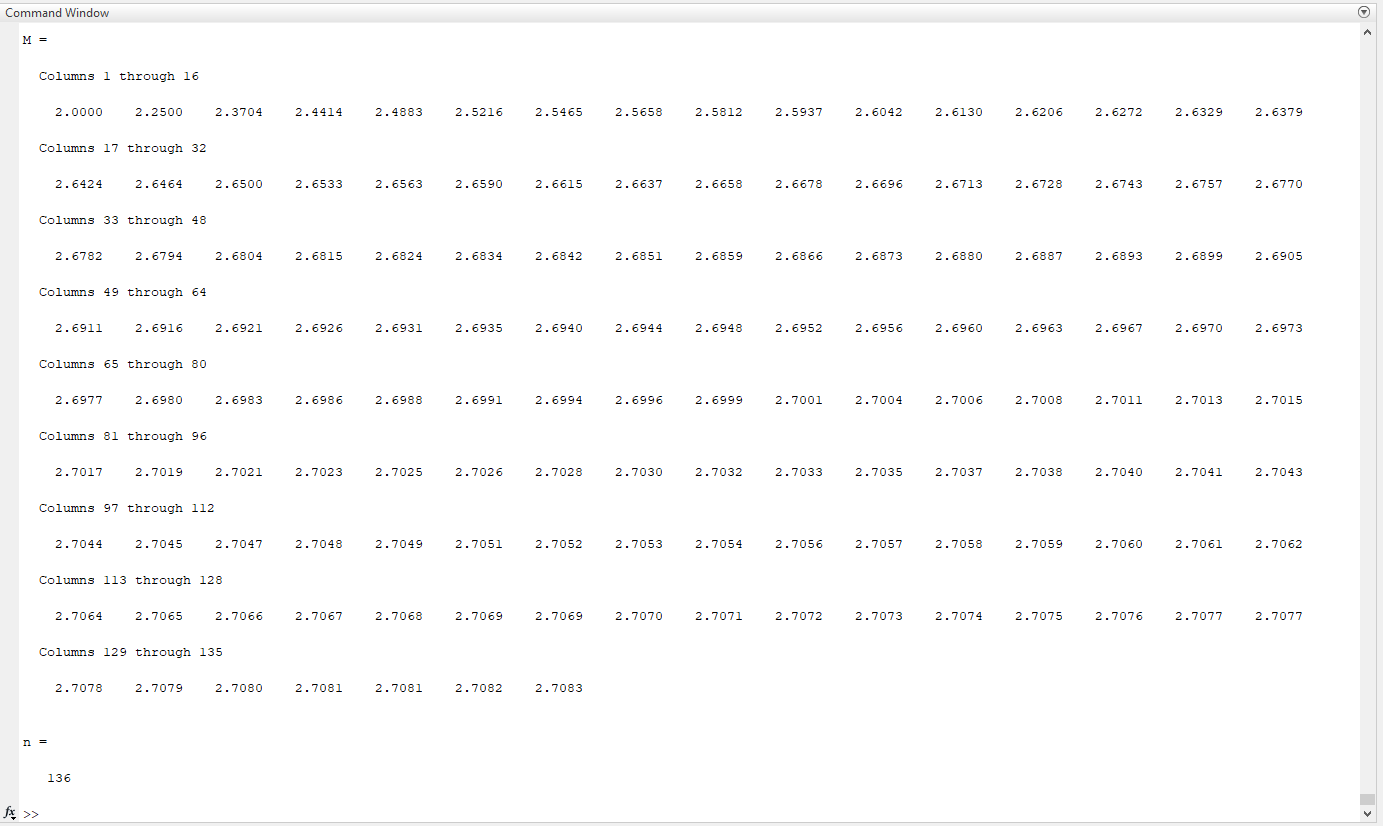
\includegraphics[scale = .5]{b.png}\\
    And one the last line, we find it took 136 iterations to be within $\epsilon = 
    10^{-2}$. Thus, our $N = 136$ 

    
    
\end{enumerate}

\end{document}